%% -*- coding: utf-8 -*-
\documentclass{beamer}

%% -*- coding: utf-8 -*-
\usetheme{Boadilla} % default
\useoutertheme{infolines}
\setbeamertemplate{navigation symbols}{} 

\usepackage{etex}
\usepackage{alltt}
\usepackage{pifont}
\usepackage{color}
\usepackage[utf8]{inputenc}
%\usepackage{german}
\usepackage{listings}
\lstset{language=Haskell}
\lstset{sensitive=true}
\usepackage{hyperref}
\hypersetup{colorlinks=true}
\usepackage[final]{pdfpages}
\usepackage{url}
\usepackage{arydshln} % dashed lines
\usepackage{tikz}
\usepackage{mathpartir}

\DeclareUnicodeCharacter{3BB}{\ensuremath{\lambda}}


\newcommand\cmark{\ding{51}}
\newcommand\xmark{\ding{55}}

\newcommand{\nat}{\mathbf{N}}

\usepackage[all]{xy}

%% new arrow tip for xy
\newdir{|>}{!/4.5pt/@{|}*:(1,-.2)@^{>}*:(1,+.2)@_{>}}

\newcommand\cid[1]{\textup{\textbf{#1}}} % class names
\newcommand\kw[1]{\textup{\textbf{#1}}}  % key words
\newcommand\tid[1]{\textup{\textsf{#1}}} % type names
\newcommand\vid[1]{\textup{\texttt{#1}}} % value names
\newcommand\Mid[1]{\textup{\texttt{#1}}} % method names

\newcommand\TODO[1][]{{\color{red}{\textbf{TODO: #1}}}}

\newcommand\String[1]{\texttt{\dq{}#1\dq{}}}

\newcommand\ClassHead[1]{%
  \ensuremath{\begin{array}{|l|}
      \hline
      \cid{#1}
      \\\hline
    \end{array}}}
\newcommand\AbstractClass[2]{%
  \ensuremath{\begin{array}{|l|}
      \hline
      \cid{\textit{#1}}
      \\\hline
      #2
      \hline
    \end{array}}}
\newcommand\Class[2]{%
  \ensuremath{\begin{array}{|l|}
      \hline
      \cid{#1}
      \\\hline
      #2
      \hline
    \end{array}}}
\newcommand\Attribute[3][black]{\textcolor{#1}{\Param{#2}{#3}}\\}
\newcommand\Methods{\hline}
\newcommand\MethodSig[3]{\Mid{#2} (#3): \,\tid{#1}\\}
\newcommand\CtorSig[2]{\Mid{#1} (#2)\\}
\newcommand\AbstractMethodSig[3]{\Mid{\textit{#2}} (#3): \,\tid{#1}\\}
\newcommand\Param[2]{\vid{#2}:~\tid{#1}}

\lstset{%
  frame=single,
  xleftmargin=2pt,
  stepnumber=1,
  numbers=left,
  numbersep=5pt,
  numberstyle=\ttfamily\tiny\color[gray]{0.3},
  belowcaptionskip=\bigskipamount,
  captionpos=b,
  escapeinside={*'}{'*},
  % language=java,
  tabsize=2,
  emphstyle={\bf},
  commentstyle=\mdseries\it,
  stringstyle=\mdseries\rmfamily,
  showspaces=false,
  showtabs=false,
  keywordstyle=\bfseries,
  columns=fullflexible,
  basicstyle=\footnotesize\CodeFont,
  showstringspaces=false,
  morecomment=[l]\%,
  rangeprefix=////,
  includerangemarker=false,
}

\newcommand\CodeFont{\sffamily}

\definecolor{lightred}{rgb}{0.8,0,0}
\definecolor{darkgreen}{rgb}{0,0.5,0}
\definecolor{darkblue}{rgb}{0,0,0.5}

\newcommand\highlight[1]{\textcolor{blue}{\emph{#1}}}
\newcommand\GenClass[2]{\cid{#1}\texttt{<}\cid{#2}\texttt{>}}

\newcommand\Colored[3]{\alt<#1>{\textcolor{#2}{#3}}{#3}}

\newcommand\nt[1]{\ensuremath{\langle#1\rangle}}

\newcommand{\free}{\operatorname{free}}
\newcommand{\bound}{\operatorname{bound}}
\newcommand{\var}{\operatorname{var}}
\newcommand\VSPBLS{\vspace{-\baselineskip}}

\newcommand\IF{\textit{IF}}
\newcommand\TRUE{\textit{TRUE}}
\newcommand\FALSE{\textit{FALSE}}

\newcommand\IFZ{\textit{IF0}}
\newcommand\ZERO{\textit{ZERO}}
\newcommand\SUCC{\textit{SUCC}}
\newcommand\ADD{\textit{ADD}}
\newcommand\SUB{\textit{SUB}}
\newcommand\MULT{\textit{MULT}}
\newcommand\DIV{\textit{DIV}}

\newcommand\PAIR{\textit{PAIR}}
\newcommand\FST{\textit{FST}}
\newcommand\SND{\textit{SND}}

\newcommand\CASE{\textit{CASE}}
\newcommand\LEFT{\textit{LEFT}}
\newcommand\RIGHT{\textit{RIGHT}}

\newcommand\Encode[1]{\lceil#1\rceil}
\newcommand\Reduce{\stackrel\ast\rightarrow_\beta}

\newcommand\Nat{\textit{Nat}}
\newcommand\Bool{\textit{Bool}}
\newcommand\Pair{\textit{Pair}}
\newcommand\Tfun[1]{#1\to}

\newcommand\Tenv{A}
\newcommand\Lam[1]{\lambda#1.}
\newcommand\App[1]{#1\,}
\newcommand\Succ{\textit{SUCC}\,}
\newcommand\Let[2]{\textit{let}\,#1=#2\,\textit{in}\,}

\newcommand\calE{\mathcal{E}}
\newcommand\calU{\mathcal{U}}
\newcommand\calP{\mathcal{P}}
\newcommand\calW{\mathcal{W}}

\newcommand\GEN{\textit{gen}}
\newcommand\EFV[1]{\textit{fv} (#1)}
\newcommand\Dom[1]{\textit{dom} (#1)}

%%% Local Variables: 
%%% mode: latex
%%% TeX-master: nil
%%% End: 

%%% frontmatter
%% -*- coding: utf-8 -*-

\title{Functional Programming}
\subtitle{Introduction}

\author[Peter Thiemann]{Prof. Dr. Peter Thiemann}
\institute[Univ. Freiburg]{Albert-Ludwigs-Universität Freiburg, Germany}
\date{SS 2021}


\usepackage{tikz}

\subtitle{Part I}
\date{Uder, 30.05.2019}

\begin{document}
\AtBeginSection[]
{
 \begin{frame}<beamer>
 \frametitle{Plan}
 \tableofcontents[currentsection]
 \end{frame}
}

\begin{frame}
  \titlepage
\end{frame}


%----------------------------------------------------------------------

% \begin{frame}
%   \frametitle{Contents}
%   \begin{itemize}
%   \item Basics of functional programming using Haskell
%   \item Haskell development tools
%   \item Writing Haskell programs
%   \item Using Haskell libraries
%   \item Your first Haskell project
%   \end{itemize}
% \end{frame}


%----------------------------------------------------------------------
\section{Introduction}
\begin{frame}
  \frametitle{What is Functional Programming?}
  \begin{block}<+->{A different approach to programming}
    \begin{LARGE}
      \begin{center}\bf
        ~
        \\[1ex]
        Functions and values
        \\[2ex]
        {\normalsize rather than}
        \\[2ex]
        Assignments and addresses
        \\[1ex]
        ~
      \end{center}
    \end{LARGE}
  \end{block}
  \begin{alertblock}<+->{\bf It will make you a better programmer}
    ~
  \end{alertblock}
\end{frame} 
%----------------------------------------------------------------------

\begin{frame}[fragile]
  \frametitle{Functional vs Imperative Programming: Variables}
  \begin{block}<+->{Functional (Haskell)}
    \begin{minipage}[t]{0.45\linewidth}
\begin{lstlisting}[language=Haskell]
x :: Int
x = 5
\end{lstlisting}
    \end{minipage}
    ~
    \begin{minipage}[t]{0.45\linewidth}
      \begin{itemize}
      \item Variable \texttt{x} has value \texttt{5} forever
      \item It's ok to replace \texttt{x} by \texttt{5} whenever needed
      \end{itemize}
    \end{minipage}
  \end{block}
  \begin{block}<+->{Imperative (Java / C)}
    \begin{minipage}[t]{0.45\linewidth}
\begin{lstlisting}[language=Java]
int x = 5;
...
x = x+1;
\end{lstlisting}
    \end{minipage}
    ~
    \begin{minipage}[t]{0.45\linewidth}
      \begin{itemize}
      \item Variable \texttt{x} can change its content over time
      \item Current value of \texttt{x} needs to be looked up in the store
      \end{itemize}
    \end{minipage}
  \end{block}
\end{frame}

\begin{frame}[fragile]
  \frametitle{Functional vs Imperative Programming: Functions}
  \begin{block}<+->{Functional (Haskell)}
    \begin{minipage}[t]{0.45\linewidth}
\begin{lstlisting}[language=Haskell]
f :: Int -> Int -> Int
f x y = 2*x + y

f 42 16 // always 100
\end{lstlisting}
    \end{minipage}
    ~
    \begin{minipage}[t]{0.45\linewidth}
      Return value of a function \textbf{only} depends on its inputs
    \end{minipage}
  \end{block}
  \begin{block}<+->{Imperative (Java)}
    \begin{minipage}[t]{0.45\linewidth}
\begin{lstlisting}[language=Java]
boolean flag;
static int f (int x, int y) {
  return flag ? 2*x + y , 2*x - y;
}

int z = f (42, 16); // who knows?
\end{lstlisting}
    \end{minipage}
    ~
    \begin{minipage}[t]{0.45\linewidth}
      Return value depends on non-local variable \texttt{flag}
    \end{minipage}
  \end{block}
\end{frame}

\begin{frame}[fragile]
  \frametitle{Functional vs Imperative Programming: Laziness}
  \begin{block}<+->{Haskell}
    \begin{minipage}[t]{0.45\linewidth}
\begin{lstlisting}[language=Haskell]
x = expensiveComputation
g anotherExpensiveComputation
\end{lstlisting}
    \end{minipage}
    ~
    \begin{minipage}[t]{0.45\linewidth}
      \begin{itemize}
      \item The expensive computation will only happen if \texttt{x}
        is ever used.
      \item Another expensive computation will only happen if
        \texttt{g} uses its argument.
      \end{itemize}
    \end{minipage}
  \end{block}
  \begin{block}<+->{Java}
    \begin{minipage}[t]{0.45\linewidth}
\begin{lstlisting}[language=Java]
int x = expensiveComputation;
g (anotherExpensiveComputation)
\end{lstlisting}
    \end{minipage}
    ~
    \begin{minipage}[t]{0.45\linewidth}
      \begin{itemize}
      \item Both expensive computations will happen anyway.
      \item Laziness can be simulated, but it's complex!
      \end{itemize}
    \end{minipage}
  \end{block}
\end{frame}

%----------------------------------------------------------------------
\begin{frame}
  \frametitle{Many features that make programs more concise}
  \begin{itemize}
  \item Pattern Matching
  \item Higher-order functions
  \item Algebraic datatypes
  \item Polymorphic types
  \item Parametric overloading
  \item Type inference
  \item Monads \& friends (for IO, concurrency, \dots)
  \item Comprehensions
  \item Metaprogramming
  \item Domain specific languages
  \item \dots
  \end{itemize}
\end{frame}
%----------------------------------------------------------------------
\section{Types}
\begin{frame}[fragile]
  \frametitle{Predefined Types}
  \framesubtitle{Every Haskell value has a type}
  \begin{center}
    \begin{tabular}{l@{ --- }l}
      \texttt{Bool}
      & \lstinline|True :: Bool|, \lstinline|False :: Bool| \\
      \texttt{Char}
      &\lstinline|'x' :: Char|, \lstinline|'?' :: Char|, \dots\\
      \texttt{Double}, \texttt{Float}
      & \lstinline|3.14 :: Double| \\
      \texttt{Integer}
      & \lstinline|4711 :: Integer| \\
      \texttt{Int}
      &machine integers ($\ge$ 30 bits signed integer) \\
      \texttt{()}
      & the \alert{unit type}, single value \lstinline|() :: ()| \\
      \lstinline|a -> b|
      & function types \\
      \lstinline|(a, b)|
      &tuple types \\
      \lstinline|[a]|
      &list types \\
      \lstinline|String|
      &  \lstinline|"xyz" :: String|, \dots
    \end{tabular}
  \end{center}
\end{frame}
% ----------------------------------------------------------------------
\begin{frame}[fragile]
  \frametitle{Functions}
\begin{block}{Examples.hs}
\begin{lstlisting}
dollarRate = 1.3671

-- |convert EUR to USD
usd euros = euros * dollarRate
\end{lstlisting}
  \end{block}
  \begin{itemize}
  \item \lstinline{dollarRate} defines a constant
  \item \lstinline{usd} is a function 
  \item Its type \lstinline{Double -> Double} is \alert{inferred} by
    the Haskell compiler
  \item To compute, a function call \lstinline{usd arg} is replaced by
    the right hand side of its definition\\
    \lstinline{usd arg} $\rightarrow$ \lstinline{arg * dollarRate}
    $\rightarrow$ \lstinline{arg * 1.3671} $\rightarrow$ \dots
  \end{itemize}
\end{frame}
%----------------------------------------------------------------------
\begin{frame}[fragile]
  \frametitle{Recursive functions}
  Compute \verb|x^n| without using the built-in operator
\begin{lstlisting}
-- compute x to n-th power
power x n | n == 0 = 1
power x n | n > 0  = x * power x (n - 1)
\end{lstlisting}
  \begin{itemize}
  \item defined using \alert{guarded equations}
  \item computation chooses the first equation such that the guard is
    true
    \begin{itemize}
    \item \lstinline|power 5 0| $\rightarrow$ \lstinline|1|
    \item \lstinline|power 5 2| $\rightarrow$
      \lstinline|5 * power 5 1| $\rightarrow$
      \lstinline|5 * (5 * power 5 0)| $\rightarrow$
      \lstinline|5 * (5 * 1)|
    \end{itemize}
  \end{itemize}
\end{frame}

% ----------------------------------------------------------------------
\begin{frame}[fragile]
  \frametitle{Tuples}
  \begin{block}{}
\begin{lstlisting}[language=Haskell]
-- example tuples
examplePair :: (Double, Bool)  -- Double x Bool
examplePair = (3.14, False)

exampleTriple :: (Bool, Int, String) -- Bool x Int x String
exampleTriple = (False, 42, "Answer")

exampleFunction :: (Bool, Int, String) -> Bool
exampleFunction (b, i, s) = not b && length s < i
\end{lstlisting}
  \end{block}
  \begin{alertblock}{Summary}
    \begin{itemize}
    \item Syntax for tuple type like syntax for tuple values
    \item Tuples are \textbf{immutable}: in fact, \textbf{all values
        are}!\\
      Once a value is defined it cannot change! 
    \end{itemize}
  \end{alertblock}
\end{frame}
%----------------------------------------------------------------------

\begin{frame}
  \frametitle{Typing for Tuples}
  \begin{block}{Typing Rule}
    \begin{mathpar}
      \inferrule[Tuple]{e_1 :: t_1 \\ e_2 :: t_2 \\\dots \\ e_n :: t_n}{
        (e_1, \dots, e_n) :: (t_1, \dots, t_n)}
    \end{mathpar}
    If
    \begin{itemize}
    \item $e_1, \dots, e_n$ are Haskell expressions
    \item $t_1, \dots, t_n$ are their respective types
    \item Then the tuple expression $(e_1, \dots, e_n)$ has the tuple
      type $(t_1, \dots, t_n)$.
    \end{itemize}
  \end{block}
\end{frame}
%----------------------------------------------------------------------

\begin{frame}
  \frametitle{Lists}
  \begin{itemize}
  \item The “duct tape” of functional programming
  \item Collections of things of the same type 
  \item 
    For any type \lstinline{a}, \lstinline{[a]} is the type of lists
    with elements of type \lstinline{a}
    \\ e.g. \lstinline{[Bool]} is the type of lists of \lstinline{Bool}
  \item Syntax for list type like syntax for list values
  \item Lists are \textbf{immutable}: once a list value is defined it cannot change!
  \end{itemize}
\end{frame}
%----------------------------------------------------------------------
\begin{frame}[fragile]
  \frametitle{Constructing lists}
  \begin{block}<+->{The values of type [a] are \dots}
    \begin{itemize}
    \item either \lstinline{[]}, the empty list
    \item or \lstinline{x:xs} where \lstinline{x} has type \lstinline{a} and
      \lstinline{xs} has type \lstinline{[a]} \\
      ``\lstinline{:}'' is pronounced ``cons''
    \item \lstinline{[]} and \lstinline{(:)} are the \textbf{list constructors}
    \end{itemize}
  \end{block}
  \begin{block}<+->{Typing Rules for Lists}
    \begin{mathpar}
      \inferrule[Nil]{}{ [] :: [t] }

      \inferrule[Cons]{e_1 :: t \\ e_2 :: [t]}{(e_1 : e_2) :: [t]}
    \end{mathpar}
    \begin{itemize}
    \item The empty list can serve as a list of any type $t$
    \item If there is some $t$ such that $e_1$ has type $t$ and $e_2$
      has type $[t]$, then $(e_1:e_2)$ has type $[t]$.
    \end{itemize}
  \end{block}
\end{frame}
%----------------------------------------------------------------------
\begin{frame}
  \frametitle{List shorthands}
  \begin{block}{Equivalent ways of writing a list}
    \begin{flushleft}
      \begin{tabular}{l@{\qquad---\qquad}l}
        \lstinline{1:(2:(3:[ ]))}& standard, fully parenthesized\\
        \lstinline{1:2:3:[ ]} & \lstinline{(:)} associates to the right\\
        \lstinline{[1,2,3]} &  bracketed notation
      \end{tabular}
    \end{flushleft}
  \end{block}
\end{frame}

%----------------------------------------------------------------------
\begin{frame}[fragile]
  \frametitle{Typing Lists}
\begin{alertblock}<+->{Quiz Time}
    Which of the following expressions have type \lstinline{[Bool]}?
\begin{lstlisting}[language=Haskell]
  [ ]
  True : [ ]
  True : False
  False : (False : [ ])
  (False : False) : [ ]
  (False : []) : [ ]
  (True : (False : (True : []))) : (False:[]):[ ]
\end{lstlisting}
  \end{alertblock}
\end{frame}
%----------------------------------------------------------------------
\section{Pattern Matching on Lists}
\begin{frame}[fragile]
  \frametitle{Functions on lists}
  \begin{block}<+->{Definition by \textbf{pattern matching}}
\begin{lstlisting}
-- double every element of a list of integers: double [3,6,12] == [6,12,24]
doubles :: [Integer] -> [Integer]
doubles []     = []
doubles (x:xs) = (2 * x) : doubles xs
\end{lstlisting}
  \end{block}
  \begin{alertblock}<+->{Argument value is checked against patterns}
    \footnotesize{}
    \begin{itemize}
    \item patterns contain constructors (\lstinline{[]} and \lstinline{:}) and variables
    \item patterns are checked in sequence; matching equation is chosen
    \item constructors are checked against argument value
    \item variables are bound to the values in
      corresponding position in the argument
    % \item each variable may occur at most once in a pattern
    % \item wild card pattern \verb!_! matches everything, no binding, may occur multiple times
    \end{itemize}
  \end{alertblock}
  \begin{block}<+->{Example evaluation}
    \lstinline{doubles (3 : 6 : 12 : [])} $\rightarrow$
    \begin{tabular}[t]{l}
    \lstinline|(2 * 3) : doubles (6 : 12 : [])| $\rightarrow$ \\
    \lstinline|6 : (2 * 6) : doubles (12 : [])| $\rightarrow$ \dots
    \end{tabular}
  \end{block}
\end{frame}
%----------------------------------------------------------------------
\begin{frame}[fragile]
    \frametitle{Higher-order functions}
    \begin{alertblock}<+->{Definition}
      A \alert{higher-order function} takes a function argument
      or returns it as a result.
    \end{alertblock}
    \begin{exampleblock}<+->{Example}
\begin{lstlisting}
twice :: (a -> a) -> (a -> a)
twice f x = f (f x)
\end{lstlisting}
      \begin{itemize}
      \item \lstinline{twice} takes a function \lstinline{f} and an
        argument and applies \lstinline{f} two times to the argument.
      \item \lstinline{(+1)} is the function that adds one to its
        argument
      \item What is \lstinline{twice (+1)}?
      \item<+-> That's the function that adds two to
        its argument!
      \item<+-> But what about \lstinline{twice twice (+1)}?
      \item<+-> Adds four!
      \end{itemize}
    \end{exampleblock}
  \end{frame}
%----------------------------------------------------------------------
\begin{frame}[fragile]
  \frametitle{map: Apply Function to Every Element of a List}
  \begin{block}<+->{Definition}
\begin{lstlisting}
-- map f [x1, x2, ..., xn] = [f x1, f x2, ..., fn]
map :: (a -> b) -> [a] -> [b]
map f []     = []
map f (x:xs) = f x : map f xs
\end{lstlisting}
    (map is in the standard Prelude - no need to define it)
  \end{block}
  \begin{exampleblock}<+->{Defining doubles using map}
\begin{lstlisting}
doubles xs = map (*2) xs
\end{lstlisting}
  \end{exampleblock}
\end{frame}
%----------------------------------------------------------------------
\begin{frame}[fragile]
  \frametitle{foldr: Reduce a List }
  % \framesubtitle{Making the pattern into a higher-order function}
  \begin{block}<+->{Abstracting over value and combining function}
\begin{lstlisting}
foldr :: (a -> b -> b) -> b -> [a] -> b
foldr op e []     = e
foldr op e (x:xs) = x `op` foldr' op e xs
\end{lstlisting}
    where
    \begin{itemize}
    \item \texttt{e :: b} is a value replacing the empty list
    \item \texttt{op :: a -> b -> b} is a combining function for list
      element and recursive call on the rest
    \end{itemize}
  \end{block}
  \begin{exampleblock}<+->{Example: many functions become one-liners with foldr}
\begin{lstlisting}
sum xs = foldr (+) 0 xs
product xs = foldr (*) 1 xs
\end{lstlisting}
  \end{exampleblock}
  \begin{alertblock}<+->{Also known as reduce}
    map $+$ reduce $=$ \href{https://en.wikipedia.org/wiki/MapReduce}{MapReduce}
  \end{alertblock}
\end{frame}
%----------------------------------------------------------------------
\section{Input and Output}
\begin{frame}[fragile]
  \frametitle{Referential transparency and substitutivity}
  \begin{block}<+->{Recall the beginning}
    \begin{itemize}
    \item Every variable and expression has just one value\\
      \textbf{referential transparency}
    \item Every variable can be replaced by its definition\\
      \textbf{substitutivity}
    \end{itemize}
  \end{block}
  \begin{block}<+->{Referential transparency enables reasoning}
\begin{lstlisting}
-- sequence of function calls does not matter
f () + g () == g () + f ()
-- number of function calls does not matter
f () + f () == 2 * f ()
\end{lstlisting}
  \end{block}
\end{frame}
%----------------------------------------------------------------------
\begin{frame}[fragile]
  \frametitle{How does IO fit in?}
  \begin{alertblock}<+->{Bad example}
    Suppose we had an operation that reads a number from the terminal
\begin{lstlisting}
input :: () -> Integer
\end{lstlisting}
    \begin{itemize}
    \item<+-> Consider
\begin{lstlisting}
let x = input () in
x + x
\end{lstlisting}
    \item<+-> Expectation: read one input and use it twice
    \item<+-> By substitutivity, this expression must behave like
\begin{lstlisting}
input () + input ()
\end{lstlisting}
      which reads two inputs!
    \item<+-> VERY WRONG!!!
  \end{itemize}
  \end{alertblock}
\end{frame}
%----------------------------------------------------------------------
\begin{frame}[fragile]
  \frametitle{The dilemma}
  \begin{block}<+->{Haskell is a pure language, but I/O is a side effect}
  \end{block}
  \begin{block}<+->{A contradiction?}
  \end{block}
  \begin{block}<+->{No!}
    \begin{itemize}
    \item Instead of performing IO operations directly, there is an
      abstract type of \textbf{IO instructions}, which get executed
      lazily by the operating system
    \item Some instructions (e.g., read from a file) return values, so the abstract IO type is parameterized over their type
    \item Keep in mind: instructions are just values like any other
  \end{itemize}
  \end{block}
\end{frame}
%----------------------------------------------------------------------
\begin{frame}[fragile]
  \frametitle{Haskell I/O}

\begin{block}<+->{The main function}
  Top-level result of a program is an IO ``instruction''.
\begin{lstlisting}
main :: IO ()
main = putStrLn "Hello World!"
\end{lstlisting}
  \begin{itemize}
  \item an instruction describes the \textbf{effect} of the program
  \item effect $=$ IO action, imperative state change, \dots
  \item Here: print a string on the terminal
  \end{itemize}
\end{block}
% \begin{block}<+->{An instruction that returns a result}
% \begin{lstlisting}
% -- defined in the Prelude
% readFile :: FileName -> IO String
% \end{lstlisting}
% \end{block}
\end{frame}
%----------------------------------------------------------------------
\begin{frame}[fragile]
  \frametitle{Kinds of instructions}
  \begin{block}<+->{Primitive instructions}
\begin{lstlisting}
-- predefined
putChar   :: Char -> IO ()
getChar   :: IO Char
writeFile :: FileName -> String -> IO ()
readFile  :: FileName -> IO String
\end{lstlisting}
and many more
  \end{block}
  \begin{block}<+->{No op instruction}
\begin{lstlisting}
return :: a -> IO a
\end{lstlisting}
    The IO instruction \lstinline{return 42} performs no IO, but yields the value 42.
  \end{block}
\end{frame}
%----------------------------------------------------------------------
\begin{frame}[fragile]
  \frametitle{Combining two instructions}
  \begin{block}<+->{The bind operator \texttt{>>=}}
    Intuition:  next instruction may depend on the output of the previous one
\begin{verbatim}
(>>=) :: IO a -> (a -> IO b) -> IO b
\end{verbatim}
    The instruction \texttt{m >>= f}
    \begin{itemize}
    \item first executes \texttt{m :: IO a} 
    \item gets its result \texttt{x :: a}
    \item applies \texttt{f :: a -> IO b} to the result
    \item to obtain an instruction \texttt{f x :: IO b} that returns a \texttt{b}
    \item and executes this instruction to return a \texttt{b}
    \end{itemize}
  \end{block}
  \begin{block}<+->{Example}
\begin{lstlisting}
readFiles f1 f2 =
   readFile f1 >>= \xs1 -> readFile f2 
\end{lstlisting}
  \end{block}
\end{frame}
%----------------------------------------------------------------------
\begin{frame}[fragile]
  \frametitle{Instructions vs functions}
  \begin{block}<+->{Functions}
    behave the same each time they called
  \end{block}
  \begin{block}<+->{Instructions}
    may be interpreted differently each time 
    they are executed, depending on context    
  \end{block}
\end{frame}
%----------------------------------------------------------------------
\begin{frame}
  \frametitle{Underlying concept: \textbf{Monad}}
  \begin{block}<+->{What's a monad?}
    \begin{itemize}
    \item abstract type for instructions that produce values
    \item built-in operators combination \lstinline{>>=} and no-op \lstinline{return}
    \item abstracts over different interpretations (computations)
    \end{itemize}
  \end{block}
  \begin{alertblock}<+->{IO is a special case of a monad}
    \begin{itemize}
    \item one very useful application for monads
    \item built into Haskell
    \item but there's more to the concept!
    \end{itemize}
  \end{alertblock}
\end{frame}
%----------------------------------------------------------------------
\begin{frame}[fragile,fragile]
  \frametitle{Intermezzo: Quicksort!}
% qsort :: Ord a => [a] -> [a]
% qsort (piv:xs) = qsort [x | x <- xs, x <= piv ] ++ piv : qsort [x | x <- xs, x >  piv ]
  \begin{exampleblock}<+->{Quicksort implementation}
\begin{lstlisting}
qsort [] = []
qsort (piv:xs) = qsort (filter (<= piv) xs) ++ piv : qsort (filter (> piv) xs)
\end{lstlisting}
  \end{exampleblock}
  \begin{itemize}
  \item \lstinline{(filter (<= piv) xs)} --- elements of \lstinline{xs}
    less than or equal to \lstinline{piv}
  \item predefined, but \dots
  \end{itemize}
  \begin{columns}
    \begin{column}{0.49\linewidth}
  \begin{exampleblock}<+->{filter implemented with foldr}
\begin{lstlisting}
filter :: (a -> Bool) -> [a] -> [a]
filter p = foldr op []
  where op x | p x = (x :)
             | otherwise = id
\end{lstlisting}
  \end{exampleblock}
\end{column}
    \begin{column}{0.49\linewidth}
  \begin{exampleblock}<+->{filter implemented with foldr}
\begin{lstlisting}
filter :: (a -> Bool) -> [a] -> [a]
filter p xs = foldr op [] xs
  where op x xs | p x = (x :) xs
                | otherwise = id xs
\end{lstlisting}
  \end{exampleblock}
\end{column}

  \end{columns}
\end{frame}
%----------------------------------------------------------------------
\section{Algebraic Datatypes}
\begin{frame}
  \frametitle{Algebraic Datatypes}
  \begin{itemize}
  \item Signature facility for defining datatypes in functional
    languages
  \item Originally introduced in the language Hope in the 1970s
  \item Describe a new datatype by declaring its \alert{constructor function}s and
    giving the type of their arguments
  \item Constructor functions do not evaluate their arguments (like the list
    constructors \lstinline{[]} and \lstinline{:})
  \item Constructors can be used for \alert{pattern matching} on the left side of
    function definitions
  \end{itemize}
\end{frame}
%----------------------------------------------------------------------
\begin{frame}[fragile]
  \frametitle{Example scenario}
  \begin{block}<+->{Model a card game}
    \begin{itemize}
    \item represent the game items!
    \item define game logic on the representations!
    \end{itemize}
  \end{block}
  \begin{center}
    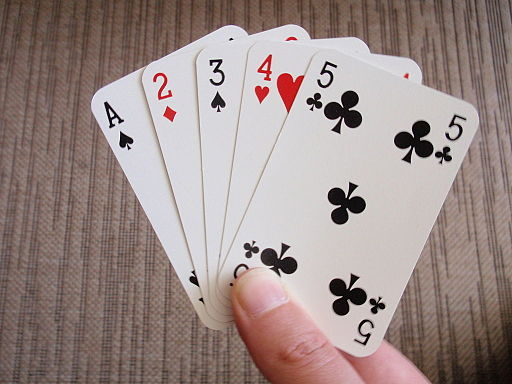
\includegraphics{pictures/AcetoFive}
  \end{center}
  \vfill
  \tiny Ron Maijen [CC BY-SA 3.0 (https://creativecommons.org/licenses/by-sa/3.0)]
  % \begin{block}<+->{Microsoft Hearts (\href{https://en.wikipedia.org/wiki/Microsoft_Hearts}{Wikipedia link})}
  %   \begin{itemize}
  %   \item computer game based on card game ``Hearts''
  %   \item included in Windows~3.1 through Windows~7
  %   \item discontinued
  %   \end{itemize}    
  % \end{block}
\end{frame}
% \begin{frame}
%   \frametitle{The game of Hearts}
%   \begin{block}<+->{Gameplay}
%     \begin{itemize}
%     \item Four players (three simulated); Trick-taking game
%     \item Each player plays one card to a trick
%     \item Trick won by highest card of the leading suit; no Trump!
%     \item Suit must be followed
%     \item Heart cannot lead until
%       \begin{itemize}
%       \item either Heart has been broken --- a player played Heart before
%       \item or the leading player has only Heart
%       \end{itemize}
%     \item Points are scored by any Heart (1 point) and the Queen of Spades (13 points) 
%     \end{itemize}
%   \end{block}
%   \begin{block}<+->{Objective}
%     \begin{itemize}
%     \item Avoid gaining points \textbf{or} gain all 26 points
%     \end{itemize}
%   \end{block}
  
% \end{frame}
%----------------------------------------------------------------------
\begin{frame}[fragile]
  \frametitle{Data model for card games}
  \begin{block}<+->{Description}
    \begin{itemize}
    \item A card has a \textbf{Suit} and a \textbf{Rank}
    \item A card beats another card if it has the same suit, but
      higher rank
    \end{itemize}
  \end{block}
  \begin{block}<+->{A card has a Suit}
\begin{lstlisting}
data Suit = Spades | Hearts | Diamonds | Clubs
\end{lstlisting}
  \end{block}
  \begin{alertblock}<+->{Explanation}
    \begin{itemize}
    \item new type consisting of four values
    \item  \texttt{Suit}: the name of the new type
    \item \texttt{Spades}, \texttt{Hearts}, \dots: the names of its
      \textbf{constructors}.
    \item Type and constructor names must be capitalized
    \end{itemize}
  \end{alertblock}
\end{frame}
% ----------------------------------------------------------------------
\begin{frame}[fragile,fragile]
  \frametitle{More data}
  A card has a suit and a \textbf{rank}:
\begin{lstlisting}
data Rank = Numeric Integer | Jack | Queen | King | Ace
\end{lstlisting}
The constructor \texttt{Numeric} is different: it takes an argument.
\begin{lstlisting}
Main> :t Numeric
Numeric :: Integer -> Rank
\end{lstlisting}
\end{frame}
%----------------------------------------------------------------------
\begin{frame}[fragile]
  \frametitle{Defining a function on Rank}
  \framesubtitle{Ordering ranks by pattern matching}
\begin{lstlisting}
-- rankBeats r1 r2 returns True, if r1 beats r2
rankBeats :: Rank -> Rank -> Bool
rankBeats _  Ace    = False
rankBeats Ace _     = True
rankBeats _ King    = False
rankBeats King _    = True
rankBeats _  Queen  = False
rankBeats Queen _   = True
rankBeats _ Jack    = False
rankBeats Jack _    = True
rankBeats (Numeric n1) (Numeric n2) = n1 > n2
--          ^^ pattern match on constructor
--             yields its argument
\end{lstlisting}

  \begin{exampleblock}<+->{Example}
\begin{lstlisting}
rankBeats Queen Jack == True
rankBeats Queen King == False
\end{lstlisting}
  \end{exampleblock}
\end{frame}
%----------------------------------------------------------------------
\begin{frame}[fragile]
  \frametitle{Datatypes can be recursive}
  \begin{block}<+->{Binary Trees}
    A binary tree is either
    \alert{empty} or  a \alert{node with a data element and two subtrees}.
\begin{lstlisting}
data BTree a = Leaf | Node (BTree a) a (BTree a)
\end{lstlisting}
  \begin{itemize}
  \item Parameterised over the type \lstinline{a} of elements
  \item Recursive datatype definition
  % \item Two arguments of \lstinline{Node} refer to the currently
  %   defined type \lstinline{BTree a}
  % \item  \lstinline{Leaf} is the \textbf{base case}
  \end{itemize}
\end{block}
\begin{exampleblock}{Example}
  \begin{minipage}{0.45\linewidth}
\begin{lstlisting}
bt :: BTree Int
bt = Node (Node Leaf 0 Leaf)
          10
          (Node Leaf 42 Leaf)
\end{lstlisting}
  \end{minipage}
  \begin{minipage}{0.45\linewidth}
    \begin{center}
      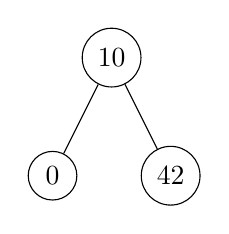
\begin{tikzpicture}
        \node[circle,draw](z){$10$} child{ node[circle,draw]{0}}
        child{ node[circle,draw]{42} };
      \end{tikzpicture}
    \end{center}
  \end{minipage}
    
\end{exampleblock}
\end{frame}
%----------------------------------------------------------------------
\section{Polymorphism and type classes}
\begin{frame}[fragile]
  \frametitle{Parametric polymorphism}
  \begin{block}<+->{Most higher-order functions are polymorphic}
\begin{lstlisting}
map    :: (a -> b) -> [a] -> [b]
filter :: (a -> Bool) -> [a] -> [a]
\end{lstlisting}
    \begin{itemize}
    \item \lstinline{a} and \lstinline{b} are \alert{type variables}
    \item the functions can be used for \textbf{any} types
      instantiated for \lstinline{a} and \lstinline{b}
    \item they work uniformly for all these instances
    \end{itemize}
  \end{block}
\end{frame}
%----------------------------------------------------------------------
\begin{frame}[fragile]
  \frametitle{Haskell integrates overloading with polymorphism}
  \begin{block}<+->{Restricted polymorphism}
    \begin{itemize}
    \item Some functions work on parametric types, but are restricted to specific instances
    \item Types contain type variables and \textbf{constraints} like
      \lstinline{Eq a}, \lstinline{Ord a} etc
    \end{itemize}
  \end{block}
  \begin{block}<+->{Examples}
\begin{lstlisting}
-- elem x xs : is x an element of list xs?
-- type a must support equality
elem :: Eq a => a -> [a] -> Bool
-- insert x xs : insert x into sorted list xs
-- type a must support comparison
insert :: Ord a => a -> [a] -> [a]
-- square x : compute the square of x
-- type a supports numeric operations
square :: Num a => a -> a
\end{lstlisting}
  \end{block}
\end{frame}
%----------------------------------------------------------------------
\begin{frame}[fragile]
  \frametitle{Type classes}
  \begin{itemize}
  \item Each constraint mentions a \textbf{type class}\\
    like \texttt{Eq}, \texttt{Ord}, \texttt{Num}, \dots
  \item A type class is a set of types that support the same operations\\
    e.g.\ members of \texttt{Eq} must support \texttt{==} and \texttt{/=}
  \item Type classes form a hierarchy\\
    e.g.\ \texttt{Eq a => Ord a} \\``must belong to \lstinline{Eq}
    before you belong to \lstinline{Ord}''
  \item Many classes are predefined, but you can roll your own
  \end{itemize}
\end{frame}
% ----------------------------------------------------------------------
\begin{frame}[fragile]
  \frametitle{Classes and Instances}
  \begin{itemize}
  \item A class declaration \textbf{only} specifies a signature (i.e., the class members and their types)
\begin{lstlisting}
class Num a where
  (+), (*), (-) :: a -> a -> a
  negate, abs, signum :: a -> a
  fromInteger :: Integer -> a
\end{lstlisting}
  \item A separate instance declaration specifies that a type belongs to a class by giving definitions for all class members
\begin{lstlisting}
instance Num Int where ...
instance Num Integer where ...
instance Num Double where ...
instance Num Float where ...
\end{lstlisting}
%   \item This info can be obtained from GHCI by
% \begin{lstlisting}
% :i Num 
% \end{lstlisting}
  \end{itemize}
\end{frame}
%----------------------------------------------------------------------
\begin{frame}[fragile]
  \frametitle{Example: Equality}
  \begin{block}<+->{The type class \texttt{Eq}}
\begin{lstlisting}
class Eq a where
  (==), (/=) :: a -> a -> Bool
  x /= y = not (x == y)         -- default definition
\end{lstlisting}
    An instance must only provide \texttt{(==)}.
  \end{block}
  \begin{alertblock}<+->{Question}
    Does equality make sense at every type?
  \end{alertblock}
\end{frame}
%----------------------------------------------------------------------
\begin{frame}[fragile]
  \frametitle{Defining \texttt{Eq} for pairs}
  \begin{block}<+->{When are two pairs equal?}
  \end{block}
  \begin{block}<+->{Solution}
\begin{lstlisting}
instance (Eq a, Eq b) => Eq (a, b) where
  (a1, b1) == (a2, b2) = a1 == a2 && b1 == b2
\end{lstlisting}
  \end{block}
  \begin{block}<+->{Is this definition recursive?}
  \end{block}
  \begin{alertblock}<+->{NO!}
  \end{alertblock}
\end{frame}
% ----------------------------------------------------------------------
\begin{frame}[fragile]
  \frametitle{Defining Eq for Suit}
  \begin{block}<+->{Manual definition}
\begin{lstlisting}
data Suit = Spades | Hearts | Diamonds | Clubs

instance Eq Suit where
  Spades == Spades = True
  Hearts == Hearts = True
  Diamonds == Diamonds = True
  Clubs == Clubs = True
  _ == _ = False // any other combination
\end{lstlisting}
  \end{block}
  \begin{alertblock}<+->{Boring to write boilerplate code \dots}
    
  \end{alertblock}
  \begin{block}<+->{Automatic derivation of Eq instance}
\begin{lstlisting}
data Suit = Spades | Hearts | Diamonds | Clubs
    deriving (Eq)
\end{lstlisting}
  \end{block}
\end{frame}
%----------------------------------------------------------------------
\begin{frame}[fragile]
  \frametitle{Abstract data types using type classes}
  \begin{itemize}
  \item Abstract data types separate the specification of the
    interface from the implementation
  \end{itemize}
  \begin{block}{Interface}
\begin{lstlisting}
class Stack s where
  push :: s a -> a -> s a
  pop  :: s a -> s a
  top  :: s a -> a
  init :: s a
\end{lstlisting}
  \end{block}
  \begin{block}{Implementation}
\begin{lstlisting}
instance Stack [] where
  push = flip (:)
  pop  = tail
  top  = head
  init = []
\end{lstlisting}
  \end{block}
\end{frame}
%----------------------------------------------------------------------
\section{Search trees and expression trees}
\begin{frame}[fragile]
  \frametitle{Search trees}
  \begin{alertblock}<+->{Definition}
    A \alert{search tree} is a binary tree such that  at each node
    \lstinline{Node l x r} the element \lstinline{x} is greater than every element in the left
    subtree \lstinline{l} and \lstinline{x} is less than every element
    in the right subtree \lstinline{r}.
  \end{alertblock}
  \begin{block}{Insert value into a search tree}
\begin{lstlisting}
insert :: Ord a => a -> BTree a -> BTree a
insert x Leaf         = Node Leaf x Leaf
insert x node@(Node l y r)
    | x < y = Node (insert x l) y r
    | x > y = Node l y (insert x r)
    | otherwise = node
\end{lstlisting}
    \begin{itemize}
    \item \lstinline{Ord a => ...} means that the type \lstinline{a}
      must admit comparison
    \end{itemize}
  \end{block}
\end{frame}
%----------------------------------------------------------------------
\begin{frame}[fragile]
  \frametitle{Expression trees}
    Arithmetic expressions comprising constants and binary operators 
  \begin{columns}
    \begin{column}{0.4\linewidth}
  \begin{block}<+->{Definition}
\begin{lstlisting}
data Term
  = Con Integer
  | Bin Term Op Term  
           
data Op
  = Add 
  | Sub
  | Mul
  | Div
\end{lstlisting}  
  \end{block}
\end{column}
\begin{column}{0.55\linewidth}
  \begin{block}<+->{Interpretation}
\begin{lstlisting}
eval              :: Term -> Integer
eval (Con n)      =  n
eval (Bin t op u) =  sys op (eval t) (eval u)

sys :: Op -> (Integer -> Integer -> Integer)
sys Add       =  (+)         
sys Sub       =  (-)
sys Mul       =  (*)         
sys Div       =  div
\end{lstlisting}  
  \end{block}
\end{column}
\end{columns}
\begin{exampleblock}<+->{Example}
  \begin{minipage}{0.45\linewidth}
\begin{lstlisting}
term = Bin (Con 40) Add (Con 2)
\end{lstlisting}
  \end{minipage}
  \begin{minipage}{0.45\linewidth}
\begin{center}\footnotesize
      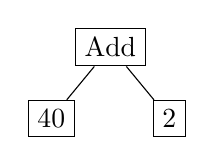
\begin{tikzpicture}[level distance=6ex]
        \node[draw](z){Add} child{ node[draw]{40}}
        child{ node[draw]{2} };
      \end{tikzpicture}
    \end{center}
  \end{minipage}
\end{exampleblock}
  \end{frame}
%----------------------------------------------------------------------
\section{Monads}
\begin{frame}[fragile]
  \frametitle{Extending the interpreter}
  \begin{block}<+->{Possible extensions}
    \begin{minipage}{0.45\linewidth}
      \begin{itemize}
      \item Error handling
      \item Counting evaluation steps
      \item Variables, state
      \item Output
      \end{itemize}
    \end{minipage}
    \begin{minipage}{0.45\linewidth}
      \only<+->{\scalebox{2}{\alert{Effects!!!}}}
    \end{minipage}

    \dots{} but without changing the structure of the interpreter!
  \end{block}
  \begin{block}<+->{Monads to the rescue}
    \begin{itemize}
    \item In each case, we can phrase the extension as a type of
      commands, as we've seen in the case of I/O.
    \item Classical FP approach to incorporate effects
    \end{itemize}
  \end{block}
\end{frame}

\begin{frame}[fragile]
  \frametitle{Commands for error handling}
  \begin{block}<+->{Interface to error handling: three operations}
    \begin{itemize}
    \item raise an error message
    \item combine computations with error handling (standard bind
      operation)
    \item return a value without an error (standard return operation)
    \end{itemize}
  \end{block}
  \begin{block}<+->{Datatype for error signaling}
\begin{lstlisting}
data Exception a =  Raise  String
                 |  Return a
\end{lstlisting}
    \begin{itemize}
    \item error messages are represented by strings
    \item \lstinline{a} is the type of normally returned values
    \end{itemize}
  \end{block}
\end{frame}
%----------------------------------------------------------------------
\begin{frame}[fragile]
  \frametitle{The Monad Interface}
\begin{block}<+->{The type class Monad}
\begin{lstlisting}
class Monad m where
  (>>=)  :: m a -> (a -> m b) -> m b
  return :: a -> m a
  fail   :: String -> m a
\end{lstlisting}
  \begin{itemize}
  \item \alert{\textbf{NEW:}} \texttt{m} is a type variable that can
    stand for \texttt{IO}, \texttt{[]}, and other \textbf{type
      constructors}. Like \lstinline{Exception}.
  \item Types of bind and return abstracted over \lstinline{IO}
  \item \lstinline{do} notation: instead of
    \lstinline{m1 >>= \x -> m2} write
\begin{lstlisting}
do x <- m1
   m2
\end{lstlisting}
  \end{itemize}
\end{block}
\end{frame}     
%----------------------------------------------------------------------
\begin{frame}[fragile]
  \frametitle{Monadic interpretation}
\begin{block}<+->{Error signaling as a monad}
\begin{lstlisting}
instance Monad Exception where
  return a = Return a
  m >>= f  = case m of 
               Raise  s -> Raise s
               Return v -> f v
  fail s   = Raise s
\end{lstlisting}
\end{block}
\begin{block}<+->{Monadic interpretation}
\begin{lstlisting}
eval             :: Term -> Exception Integer
eval (Con n)      = return n
eval (Bin t op u) = do
  v <- eval t
  w <- eval u
  if (op == Div && w == 0) 
    then fail "div by zero"
    else return (sys op v w)
\end{lstlisting}
\end{block}
  
\end{frame}
%----------------------------------------------------------------------
\begin{frame}
  \frametitle{Why would you write an interpreter in this style?}
  \begin{itemize}
  \item Easy modification to support other effects / monads.
  \item It's possible to combine monads modularly to support
    combinations of effects.
  \end{itemize}
\end{frame}
%----------------------------------------------------------------------
\begin{frame}[fragile]
  \frametitle{A monad for counting}
  \begin{block}{The state monad}
\begin{lstlisting}
data ST s a = ST (s -> (a, s))
exST (ST sas) = sas

instance Monad (ST s) where
  return a = ST (\s -> (a, s))
  m >>= f  = ST (\s -> let (a, s') = exST m s in exST (f a) s')

-- primitive for reading and writing the state
get :: ST s s
get = ST (\s -> (s, s))

put :: s -> ST s ()
put s = ST (const ((), s))

type Count a = ST Integer a

incr :: Count ()
incr = get >>= \i -> put (i+1)
\end{lstlisting} 
\end{block}
\end{frame}
% ----------------------------------------------------------------------
\begin{frame}[fragile]
  \frametitle{Monadic interpreter with reduction count}
  \framesubtitle{Implementation}
\begin{exampleblock}{Evaluation}
\begin{lstlisting}
eval :: Term -> Count Integer
eval (Con n)      = return n
eval (Bin t op u) = do
  v <- eval t
  w <- eval u
  incr
  return (sys op v w)
\end{lstlisting} 
\end{exampleblock}
\end{frame}
% ----------------------------------------------------------------------
\begin{frame}[fragile]
  \frametitle{Typical monads}
  \begin{block}<+->{Already used}
  \begin{itemize}       
  \item Identity monad
  \item Exception monad
  \item State monad
  \item I/O monad
  \end{itemize} 
\end{block}
\begin{block}{Others}
  \begin{itemize}
  \item Writer monad: supports an output operation\\
    \lstinline{Monoid w => Monad (Writer w)} where
    \lstinline{data Writer w a = Writer a w}
  \item Maybe monad: computation that may or may not return a result
  \item List monad: Multiple results / nondeterminism, backtracking
  \end{itemize}
\end{block}
\end{frame}

%----------------------------------------------------------------------
\begin{frame}[fragile]
  \frametitle{Modular computations}
  \begin{itemize}
  \item Types given to \lstinline{eval} restrict to a single monad
  \item Better to just state requirements on the monad
  \end{itemize}
  \begin{exampleblock}{Modular evaluation}
\begin{lstlisting}
incr :: MonadState Integer m => m ()
incr = get >>= \i -> put (i+1)

eval :: (MonadState Integer m, MonadError String m)
     => Term -> m Integer
eval (Con n)      = return n
eval (Bin t op u) = do
  v <- eval t
  w <- eval u
  incr
  if (op == Div && w == 0) 
    then throwError "div by zero"
    else return (sys op v w)
\end{lstlisting}
  \end{exampleblock}
\end{frame}
%----------------------------------------------------------------------
\begin{frame}
  \frametitle{Conclusion}

  \begin{block}{Still to come}
    \begin{itemize}
    \item Yet more typing features
      \begin{itemize}
      \item polymorphic functions as parameters
      \item type-level computation (associated classes and type
        families)
      \item dependent types 
      \end{itemize}
    \item Concurrency, parallelism, GPU programming
    \item Metaprogramming
    \item Domain specific languages
    \item \dots
    \end{itemize}
  \end{block}
  \begin{alertblock}{Industrial users of Haskell}
    \url{https://wiki.haskell.org/Haskell_in_industry}
  \end{alertblock}
\end{frame}
%----------------------------------------------------------------------
\begin{frame}
  \frametitle{References}
  \begin{itemize}
  \item Paper by the original developers of Haskell in the conference on History of
    Programming Languages (HOPL III): \href{A History
      of Haskell: Being Lazy with
      Class}{http://dl.acm.org/citation.cfm?id=1238856}
  \item The Haskell home page: \url{http://www.haskell.org}
  \item Haskell libraries repository:
    \url{https://hackage.haskell.org/}
  \item Haskell Tool Stack:
    \url{https://docs.haskellstack.org/en/stable/README/}
  \item The complete lecture materials
    \url{https://github.com/proglang/FunctionalProgramming}
  \end{itemize}
\end{frame}

%----------------------------------------------------------------------

% \begin{frame}
%   % \frametitle{Questions?}
%   \begin{center}
%     \tikz{\node[scale=5] at (0,0){Thank you!};}
%   \end{center}
% \end{frame}



\end{document}

%%% Local Variables: 
%%% mode: latex
%%% TeX-master: t
%%% End: 
